% !Mode:: "TeX:UTF-8"

%要运行该模板,LaTex需要安装CJK库以支持汉字.
%字体大小为12像素,文档类型为article
%如果你要写论文,就用report代替article
%所有LaTex文档开头必须使用这句话
\documentclass[12pt,twocolumn]{article}

%使用支持汉字的CJK包
\usepackage{CJKutf8}
\usepackage{indentfirst}
\usepackage[top=0.5in, bottom=0.5in, left=0.4in, right=0.4in]{geometry}
\usepackage[square,comma,numbers,sort&compress]{natbib}
\usepackage{graphicx}
\usepackage{booktabs}
\usepackage{tabularx}
\usepackage{enumitem}
\usepackage{titling}

\setlength{\parindent}{2em}
\setlength{\parskip}{0.5em}

\renewcommand{\contentsname}{目录}
\renewcommand{\listfigurename}{插图目录}
\renewcommand{\listtablename}{表格目录}
\renewcommand{\refname}{参考文献}
\renewcommand{\abstractname}{摘要}
\renewcommand{\indexname}{索引}
\renewcommand{\tablename}{表}
\renewcommand{\figurename}{图}

\setlength{\abovecaptionskip}{0em plus 0.3em minus 0.3em}
\setlength{\belowcaptionskip}{0em plus 0.3em minus 0.3em}
\setlength{\tabcolsep}{0.5em}
\setlength{\columnsep}{0.4in}

\linespread{1.1}

\setlist[1]{itemsep=0em,topsep=0em}

\renewcommand{\arraystretch}{1.3}

% make title left
\makeatletter
\renewcommand{\maketitle}{\bgroup\setlength{\parindent}{0pt}
\begin{flushleft}
  \LARGE {\textbf{\@title}}\vspace{1em}

  \normalsize{\@author}
\end{flushleft}\egroup
}
\makeatother

% change margin
\def\changemargin#1#2{\list{}{\rightmargin#2\leftmargin#1}\item[]}
\let\endchangemargin=\endlist

%开始CJK环境,只有在这句话之后,你才能使用汉字
%另外,如果在Linux下,请将文件的编码格式设置成GBK
%否则会显示乱码
\begin{CJK*}{UTF8}{gbsn}
\CJKindent
\CJKtilde

%这是文章的时间
%如果没有这行将显示当前时间
%如果不想显示时间则使用 \date{}
\date{}

%以上部分叫做"导言区",下面才开始写正文
\begin{document}

\twocolumn[
  \begin{@twocolumnfalse}
    %这是文章的标题
    \title{平行坐标综述}
    %这是文章的作者
    \author{赖楚凡\hspace{1em}袁晓如}
    %先插入标题
    \maketitle
    %\vspace{-4em}

    \begin{changemargin}{0.2in}{0in}
    {\bf 摘\hspace{1em}要:}
    \vspace{1em}

    {\bf 关键词:}
    \vspace{1em}
    \end{changemargin}

    %这是文章的标题
    \title{Parallel Coordinates}
    %这是文章的作者
    \author{Chufan Lai\hspace{1em}Xiaoru Yuan}
    %先插入标题
    \maketitle
    %\vspace{-4em}

    \begin{changemargin}{0.2in}{0in}
    {\bf Abstract: } 
    \vspace{1em}

    {\bf Keywords: }
    \vspace{2em}
    \end{changemargin}
  \end{@twocolumnfalse}
]

%再插入目录
%\tableofcontents
\section{引言}
\label{section:introduction}

在现实世界中,同一事物往往有多个不同的属性,要完整地描述该事物,需要记录其各个属性的信息。而这类具有多属性(维度)信息的数据,就称为多变量数据(Multivariate Data),或称高维数据(High-dimensional Data)。在传统的数据分析中,高维数据一般利用统计方法加以处理,并通过表格的方式呈现。但传统方法过于依赖自动算法,既无法结合用户的知识与判断,也不利于对抽象的高维信息的认知和理解。而信息可视化技术(Information Visualization)通过对高维数据的视觉呈现,辅以交互式的数据处理手段,能使用户充分参与到数据分析过程中,既加深了用户对数据的理解,也提高了分析的效率和可靠性。

高维数据一直是信息可视化领域的研究重点之一,其独有的两个特性:即维度数高、抽象性强,为可视化设计带来了巨大挑战。一方面,维度数的增长使得数据的信息量急剧增大,有限的显示空间只能表达一部分数据特征,而自动算法也会因为所谓的“维数灾难”(过高的复杂度、过低的采样率等~\citep{Bellman1962})而难以应用。另一方面,由于人无法感知高于三维的拓扑空间,高维的数据特征(如聚类、流型等)往往抽象而难以理解。针对这些挑战,领域内提出了各类高维可视化方法~\citep{grinstein2001high},包括降维投影~\citep{fodor2002survey}、散点图矩阵~\citep{cleveland1988dynamic}、雷达图~\citep{hoffman1999dimensional}、星型坐标~\citep{kandogan2000star}等等。而由Inselberg等人提出的平行坐标~\citep{inselberg1985plane}(如图\ref{fig:PC_demo})也因其简单直观、可拓展性强等优点而被广泛应用于高维数据的可视分析中。

\begin{figure}[htb!]
\centering
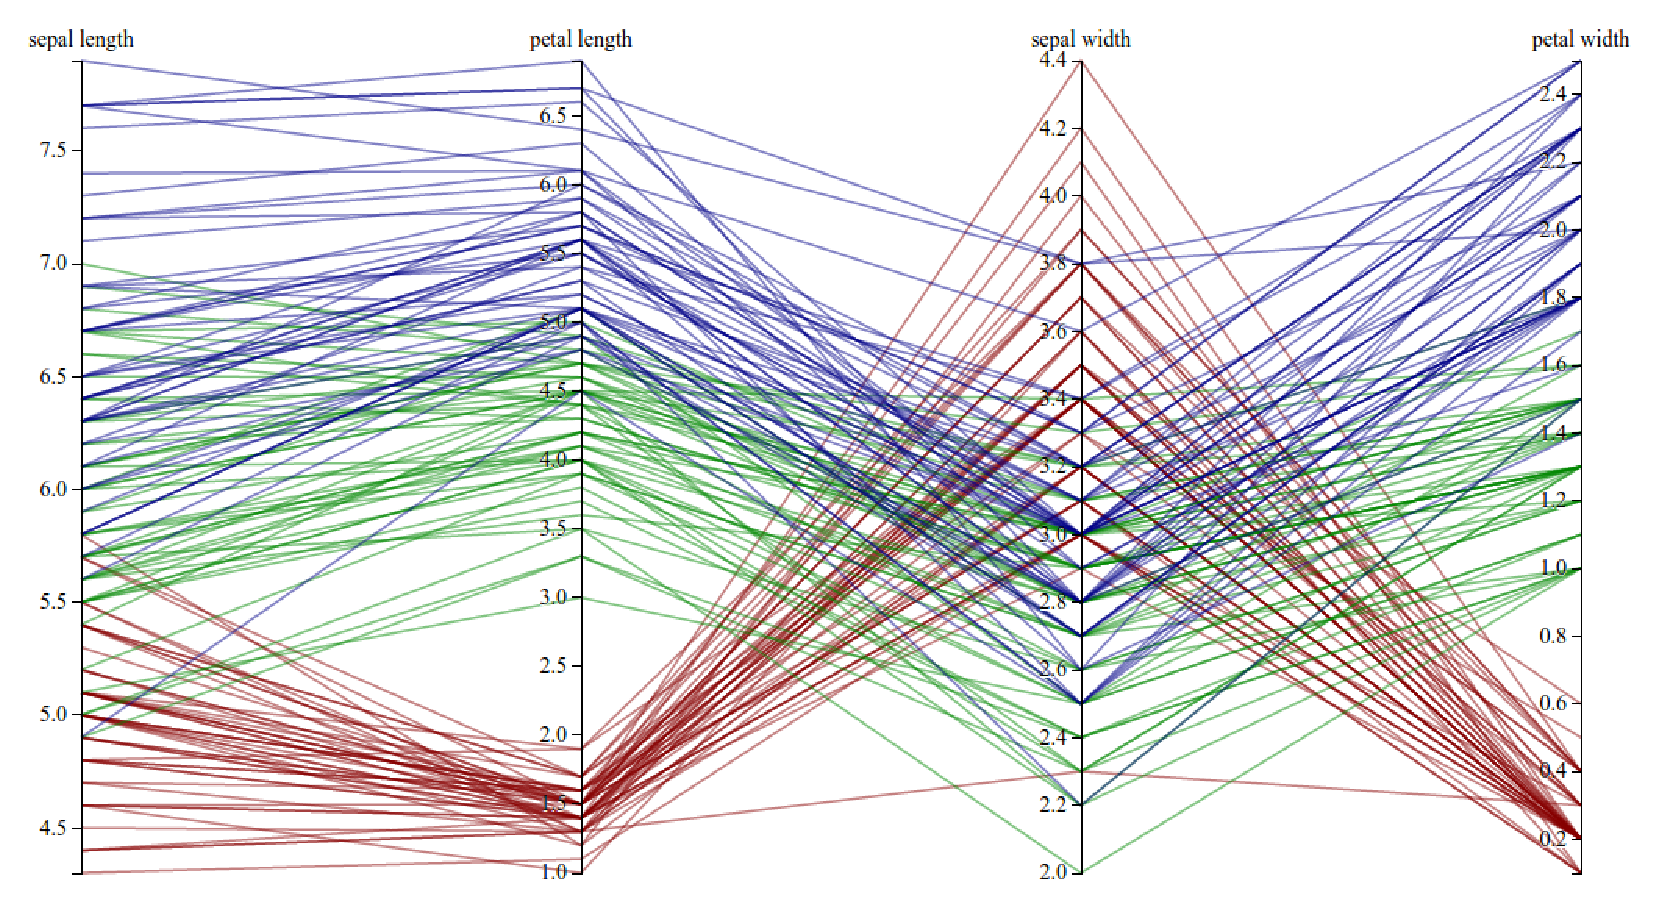
\includegraphics[width=1.0\linewidth]{images/PC_demo.eps}
\caption{\label{fig:PC_demo}平行坐标示例
}
\end{figure}

然而,相比于其他高维可视化形式,平行坐标的设计也存在种种缺点,譬如展现的信息量较少、容易出现视觉混杂(Visual Clutter)、数据特征不直观等等(详见第\ref{section:impro}节)。针对这些问题,领域内的学者们做了大量的研究工作,并提出了各种方法对平行坐标进行改进和延展。

本文基于已有的一些综述论文~\citep{heinrich2013state},并结合近年来的最新进展,将对平行坐标方面的研究工作进行比较、总结和展望。在文章的余下部分里:第\ref{section:basics&prob}节介绍了平行坐标的基本原理,并阐述其设计上存在的主要问题;第\ref{section:impro}节就平行坐标的不同部分,回顾了领域学者们为解决前述问题所作出的研究努力;第\ref{section:applications}节则介绍了平行坐标在不同领域内的应用现状;第\ref{section:challenges}节基于已有的研究和应用,探讨了仍然存在的挑战,以展望未来的研究动向和应用前景;最后,第\ref{section:conclusion}节对全文内容进行总结。

\section{基本原理及主要问题}
\label{section:basics&prob}
在这一节里,我们将简要介绍平行坐标的基本原理,包括其视觉设计和基本的交互功能。在此过程中,我们将逐步阐述平行坐标的几个主要问题。

\subsection{视觉设计}
\label{basics}
正如前节所述,人无法感知高于三维的拓扑关系。传统的笛卡尔坐标系限定了坐标轴之间必须相互垂直,这使得高维的坐标空间极为抽象和难以理解。而平行坐标解决这一难题的方法,顾名思义,就是将各个维度的坐标轴平行放置,如图\ref{fig:PC_principle}所示。一个高维数据在各个坐标轴上均有取值,连接各取值所形成的一条折线,即表达了这个数据。

\begin{figure}[!htb]
\centering
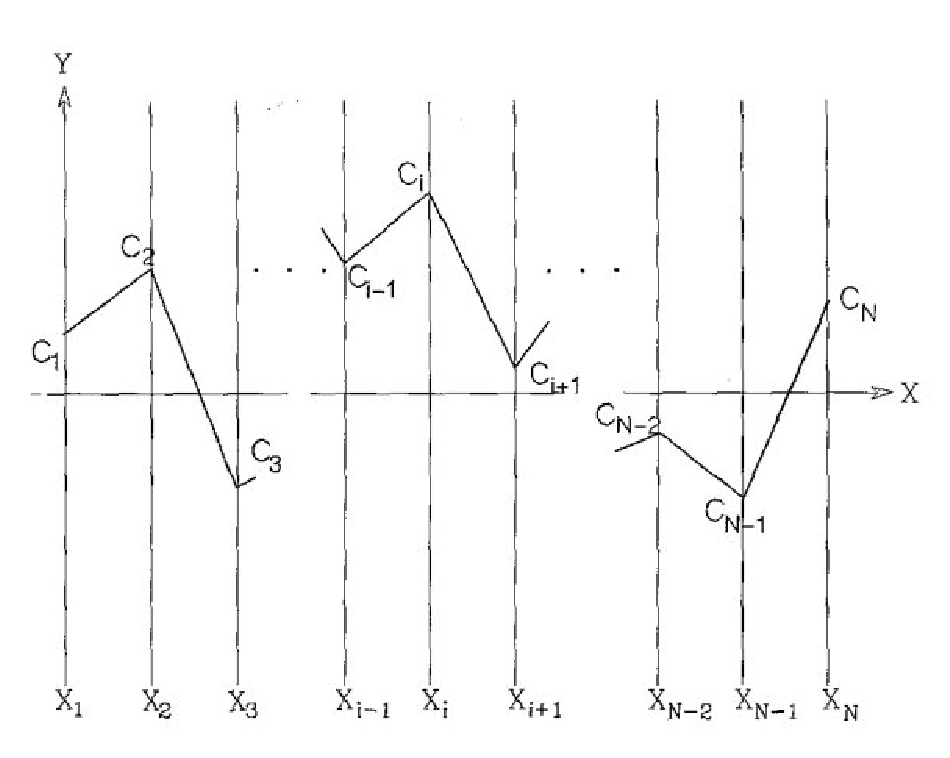
\includegraphics[width=1.0\linewidth]{images/PC_principle.eps}
\caption{\label{fig:PC_principle}平行坐标的基本原理。本图来源于Inselberg~等人的论文~\citep{inselberg1985plane}~。
}
\end{figure}

相比于其他高维可视化方法,平行坐标

\subsection{基本交互}

\section{平行坐标的改进}
\label{section:impro}

\section{平行坐标的应用}
\label{section:applications}

\section{探讨与展望}
\label{section:challenges}

\section{结论}
\label{section:conclusion}

\bibliographystyle{abbrvnat}
%\setcitestyle{aysep={,},yysep={;}}
\bibliography{parallelcoordinates}
	
\end{CJK*}
\end{document}

